\documentclass[12pt,a4paper]{article}
\usepackage{algorithm, algpseudocode, amsmath, amssymb, amsthm, csquotes, empheq, geometry, graphicx, hyperref, listings, multirow, siunitx, subcaption, upgreek}
\usepackage[italicdiff]{physics}
\usepackage[section]{placeins}
\usepackage[justification=centering]{caption}

\title{Computational Physics\\Problem Set 6}
\author{Saleh Shamloo Ahmadi\\Student Number: 98100872}
\date{November 1, 2021}

\hypersetup{colorlinks=true, urlcolor=cyan}
\newcommand{\fig}{../fig}
\newcommand{\ddfrac}[2]{{\displaystyle\frac{\displaystyle #1}{\displaystyle #2}}}

\begin{document}
	\maketitle
    \section{Central Limit Theorem}
    The central limit theorem states that the sum of independent random variables tends towards a normal distribution.
    Specifically, if $X_1, X_2, \dots, X_n$ are n random samples from a population with overall mean $\mu$ and finite
    variance $\sigma ^{2}$, and if $\bar{X}_{n}$ is the sample mean, then the limiting form of the distribution
    \begin{equation}
        Z=\lim _{n\to\infty}\frac{\sqrt{n}}{\sigma}\qty(\bar{X}_{n}-\mu)
    \end{equation}
    is a standard normal distribution, which is
    \begin{equation}
        \mathcal{N}(0, 1) = \frac{e^{-\flatfrac{x^2}{2}}}{\sqrt{2\pi}}.
    \end{equation}
    In the following figures, I generated random numbers between 0 and 1 and then compared the results (sample sums)
    to a perfect normal distribution with the same mean and variance as the generated sample.
    As you can see, the distribution of the sample is very close to a normal distribution in all
    cases, and as $N$ grows, the distribution becomes more similar to a normal distribution.

    Note that random walk generates a normal distribution exactly because of this theorem; The final position of the
    walker is the sum of a random sample from the numbers $-1$ and $1$. Each $X_n$ corresponds to a $-1$ or $1$ and
    the probability of each step is independent from other steps.
    \begin{figure}
        \centering
        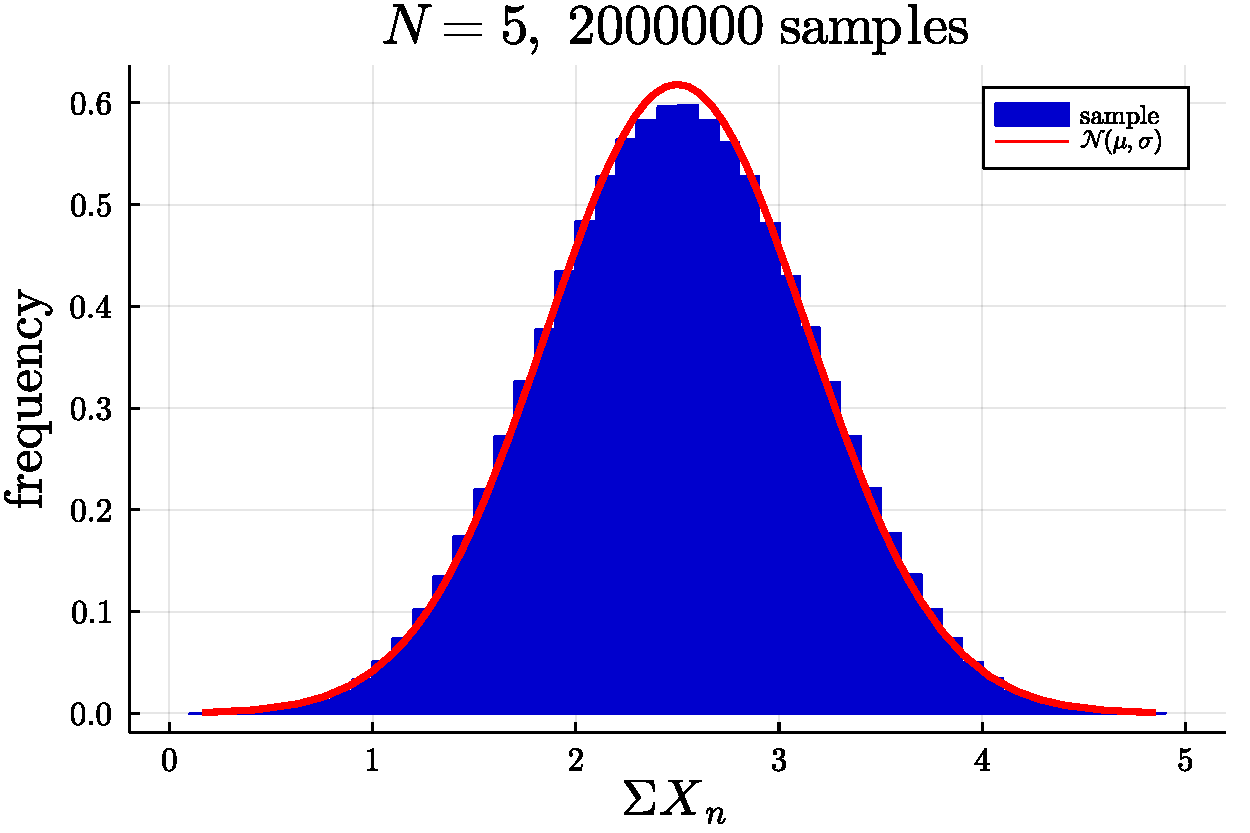
\includegraphics[width=\linewidth]{\fig/normal-5}
    \end{figure}
    \begin{figure}
        \centering
        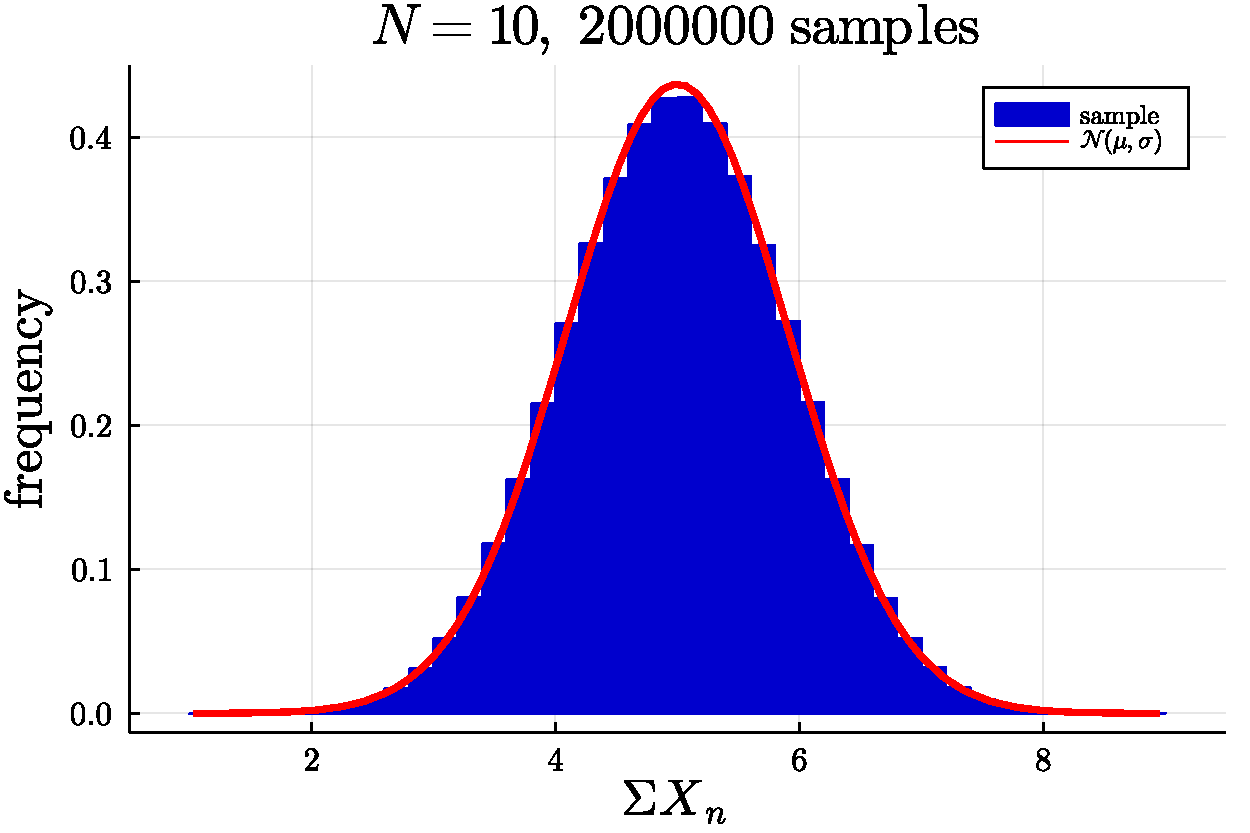
\includegraphics[width=\linewidth]{\fig/normal-10}
    \end{figure}
    \begin{figure}
        \centering
        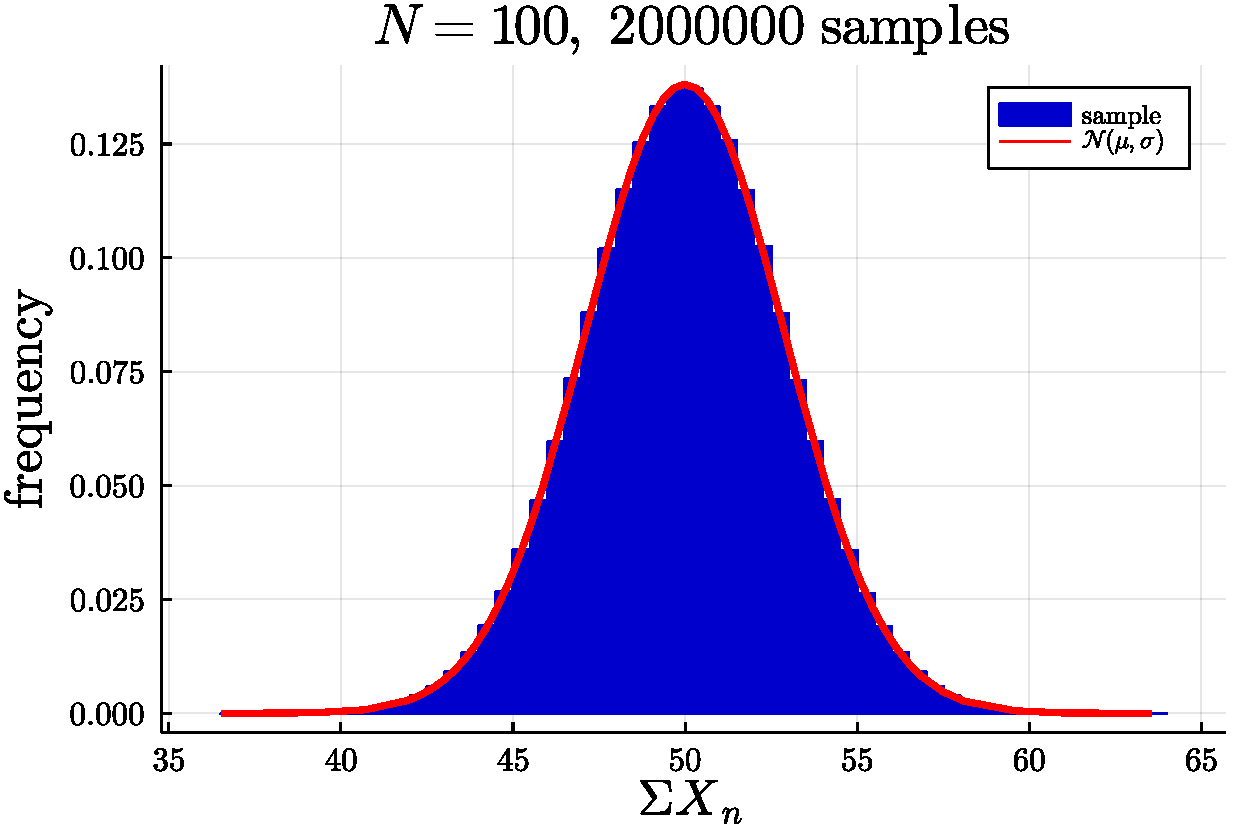
\includegraphics[width=\linewidth]{\fig/normal-100}
    \end{figure}
    \begin{figure}
        \centering
        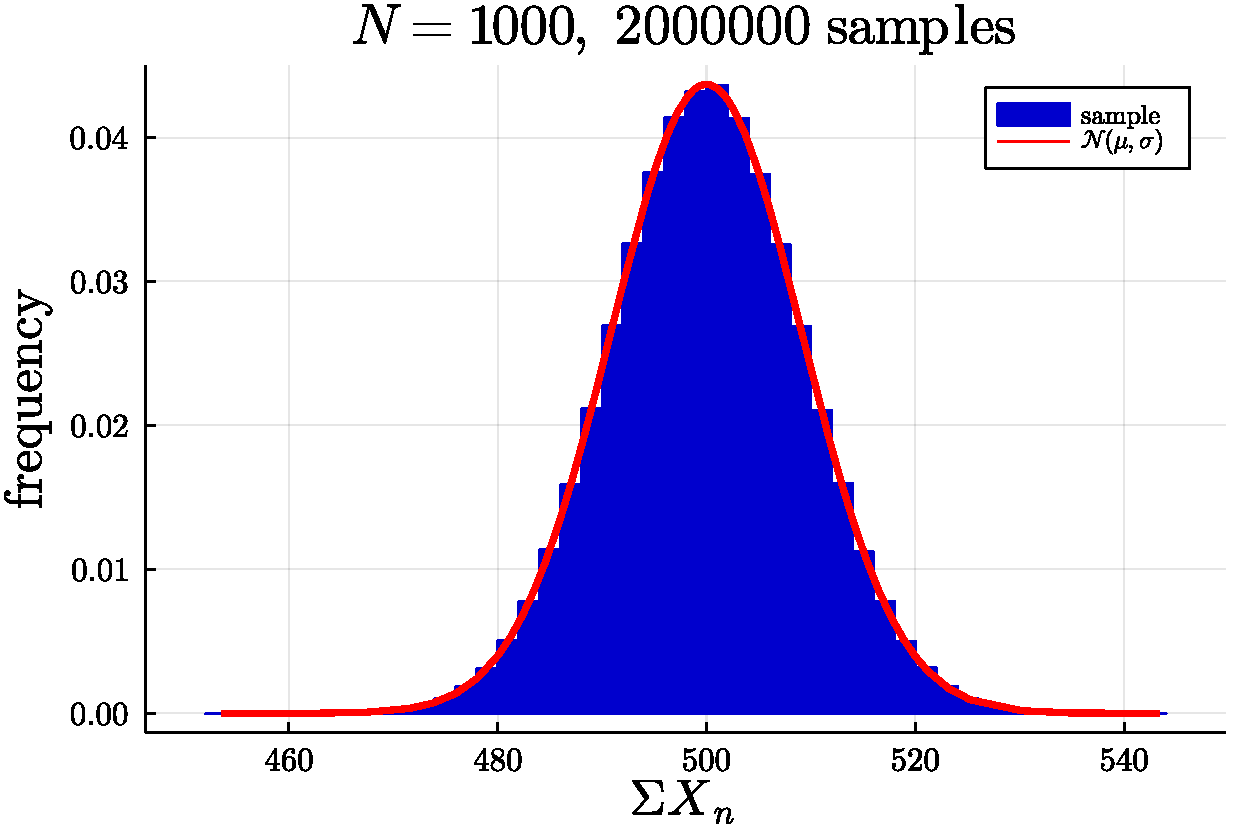
\includegraphics[width=\linewidth]{\fig/normal-1000}
    \end{figure}

    \section[Generating a Gaussian Distribution with an RNG]
    {Generating a Gaussian Distribution with an RNG\footnote{Random Number Generator}}
    The probability density function of a random number generator is constant in the range $[0,1]$ and zero elsewhere.
    If the probability density function of a random variable $x$ is given by the function $f(x)$, then with a change of
    variables $y$ can be chosen as a function of $x$ such that the probability density function of $y$ is the arbitrary
    normalized function $g(y)$; The probability of associated $x$ and $y$ is equal, so
    \begin{equation}
        f(x)\dd{x} = g(y)\dd{y} \implies \int_{-\infty}^x f(x)\dd{x} = \int_{-\infty}^y g(y)\dd{y}.
    \end{equation}
    If $x$ is generated by an RNG, then
    \begin{equation}
        x = \int_{-\infty}^y g(y)\dd{y} = G(y)
    \end{equation}
    since $G(y)$ is monotonically increasing ($g(y) > 0$, because it is a probability density function),
    it is invertible and
    \begin{equation}
        y = G^{-1}(x).
    \end{equation}

    For a gaussian (normal) distribution
    \begin{equation}
        g(y) = \ddfrac{e^{-\frac{y^2}{2\sigma^2}}}{\sqrt{2\pi\sigma^2}}.
    \end{equation}
    In this form, $G(y)$ cannot be expressed in elementary functions. to solve this issue, we can generate two random
    numbers $y_1$ and $y_2$ from $x$ instead of one:
    \begin{equation}
        g(y_1, y_2)\dd{y_1}\dd{y_2} = g(y_1)g(y_2)\dd{y_1}\dd{y_2}
        = \ddfrac{e^{-\frac{y_1^2 + y_2^2}{2\sigma^2}}}{2\pi\sigma^2}\dd{y_1}\dd{y_2}
    \end{equation}
    With a change of coordinates to polar coordinates
    \begin{gather}
        \left\{
            \begin{aligned}
                y_1 = \rho\sin{\theta}\\
                y_2 = \rho\cos{\theta}
            \end{aligned}
        \right. \\
        g(y_1, y_2)\dd{y_1}\dd{y_2} = g(\rho, \theta)\rho\dd{\rho}\dd{\theta}
        = \ddfrac{e^{-\frac{\rho^2}{2\sigma^2}}}{2\pi\sigma^2}\rho\dd{\rho}\dd{\theta}
    \end{gather}
    For normalized distributions in terms of $\rho$ and $\theta$, we can use
    \begin{empheq}[left=\empheqlbrace]{align}
        g_1(\rho) &= \ddfrac{e^{-\frac{\rho^2}{2\sigma^2}}}{\sigma^2}\rho \\
        g_2(\theta) &= \frac{1}{2\pi}
    \end{empheq}
    Now, two random numbers with gaussian distribution $y_1$ and $y_2$ can be generated from two random numbers form RNG
    $x_1$ and $x_2$:
    \begin{empheq}[left=\empheqlbrace]{align}
        G_1(\rho) &= \int_0^\rho \ddfrac{e^{-\frac{\rho^2}{2\sigma^2}}}{\sigma^2}\rho\dd{\rho}
        = 1-e^{-\frac{\rho^2}{2\sigma^2}} \\
        G_2(\theta) &= \int_0^\theta \frac{1}{2\pi}\dd{\theta} = \frac{\theta}{2\pi}
    \end{empheq}
    \begin{empheq}[left=\empheqlbrace]{align}
        \rho &= G_1^{-1}(x_1) = \sigma\sqrt{2\ln(\frac{1}{1-x_1})} \\
        \theta &= G_2^{-1}(x_2) = 2\pi x_2
    \end{empheq}
    \begin{empheq}[box=\fbox, left=\empheqlbrace]{align}
        y_1 &= \sigma\sin(2\pi x_2)\sqrt{2\ln(\frac{1}{1-x_1})} \\
        y_2 &= \sigma\cos(2\pi x_2)\sqrt{2\ln(\frac{1}{1-x_1})}
    \end{empheq}
    To create a normal distribution with mean $\mu$ and variance $\sigma^2$ it suffices to add $\mu$ to $y_1$ and $y_2$.
    \begin{figure}
        \centering
        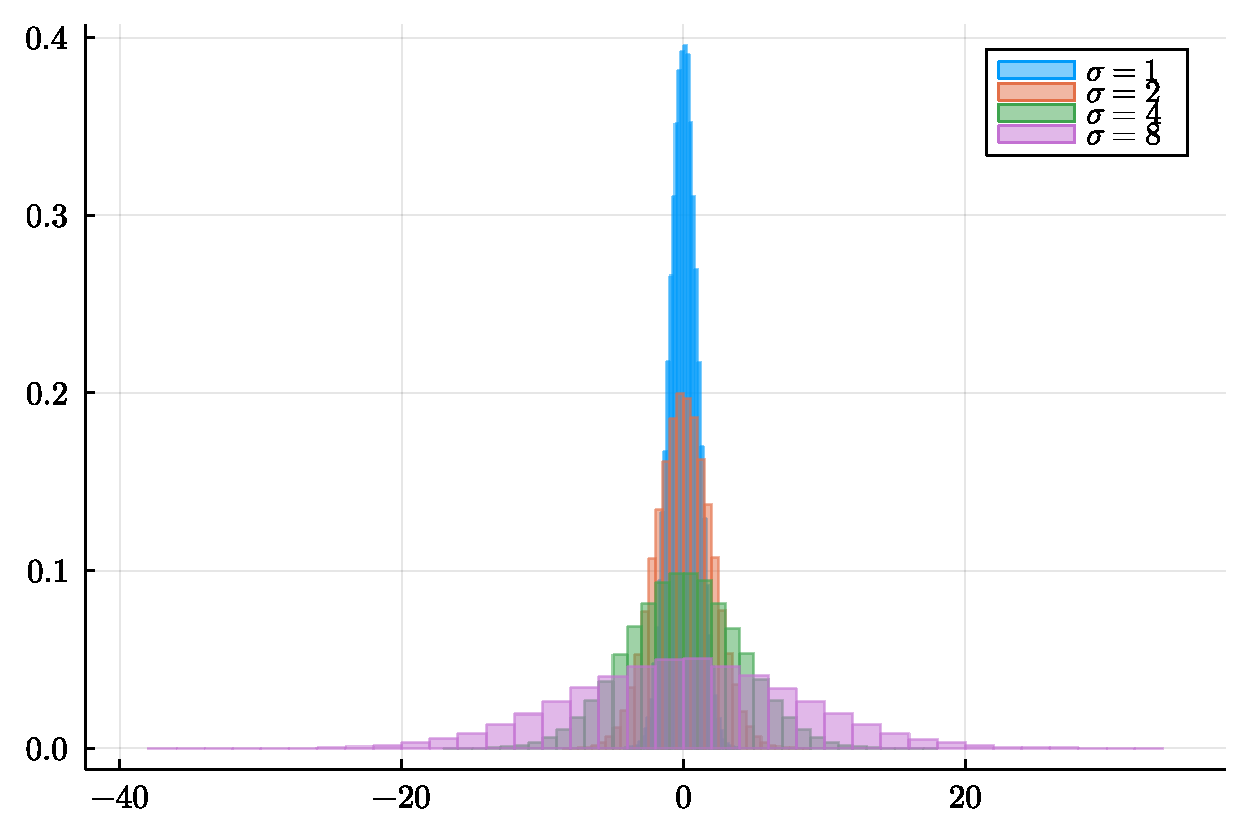
\includegraphics[width=\linewidth]{\fig/gaussian-overlay}
    \end{figure}
    \begin{figure}
        \centering
        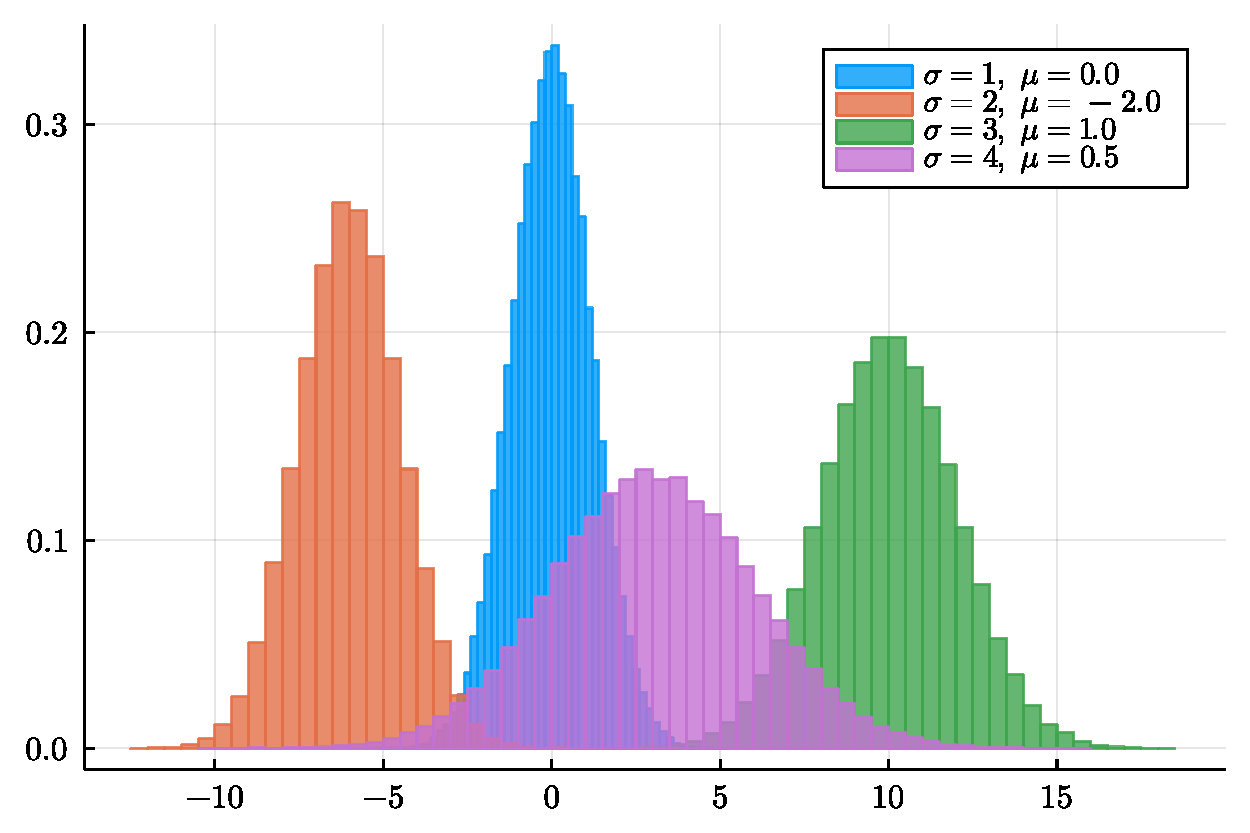
\includegraphics[width=\linewidth]{\fig/gaussian-spread}
    \end{figure}
    \begin{figure}
        \centering
        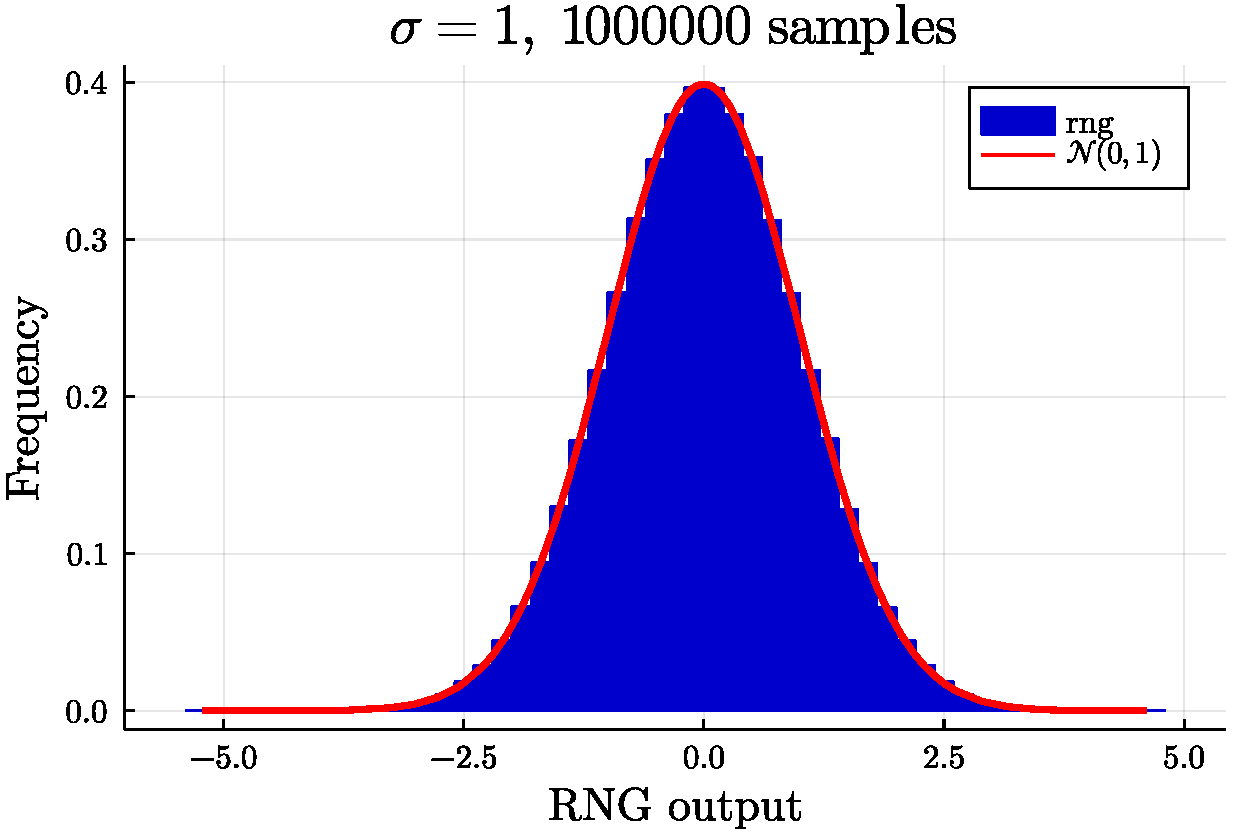
\includegraphics[width=\linewidth]{\fig/gaussian-check}
    \end{figure}
\end{document}
